\documentclass[10pt]{beamer}
\usepackage{float}
\usepackage{hyperref}
\usepackage{algorithmicx}
\usepackage{algorithm}
\usepackage{algpseudocode}
\usepackage{amsfonts}
\usepackage{amsmath}
\usepackage{bm}
\usepackage{caption}
\usepackage{color}
\usepackage{graphicx}
\usepackage{listings}
\usepackage{subcaption}
\usepackage{wrapfig}
\usepackage[backend=bibtex]{biblatex}
\usepackage[lithuanian]{babel}
\usepackage{microtype}

\renewcommand\lstlistingname{kodas}
\renewcommand{\figurename}{pav}

\usetheme[progressbar=frametitle]{metropolis}
\logo{\raisebox{-0.5cm}{
\includegraphics[width=1cm]{img/beamer-logo.png}}\hspace*{\textwidth}}
\usepackage{appendixnumberbeamer}

\usepackage{booktabs}
\usepackage[scale=2]{ccicons}

\usepackage{pgfplots}
\usepgfplotslibrary{dateplot}

\usepackage{xspace}
\newcommand{\themename}{\textbf{\textsc{metropolis}}\xspace}

\title{Žinių grafų užklausa naudojant užklausų kalbą SPARQL}
\subtitle{Querying knowledge graphs using query language SPARQL}
\date{}
\author{Tomas Kozakas}
\institute{Matematikos ir informatikos fakultetas}

\addbibresource{bibliografija.bib} 
\setbeamercolor{background canvas}{bg=white}
\begin{document}
\pagecolor{white}
\maketitle

\begin{frame}{Turinys}
  \setbeamertemplate{section in toc}[sections numbered]
  \tableofcontents
\end{frame}

\section{Įvadas}

\section{Žinių grafai}

\begin{frame}[fragile]{Apibrėžimas}
    Žinių grafas yra kryptinis grafas, kuriame taškų vardai turi aiškiai apibrėžtas reikšmes. Kryptinis grafas susideda iš taškų (nodes), briaunų (edges) ir taškų vardų \cite{stanford_what_2021}.
    \begin{figure}[htbp]
        \centering
        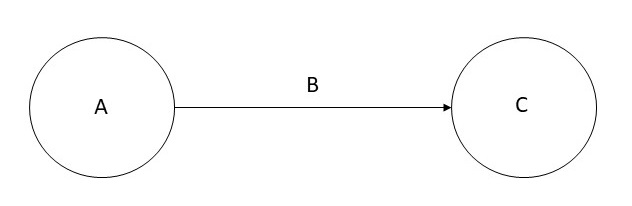
\includegraphics[width=0.5\textwidth]{img/triple.jpg}
        \label{fig:triple}
    \end{figure}
\end{frame}

\begin{frame}[fragile]{Facebook reklamos skelbimai}
    \begin{figure}[htbp]
          \centering
          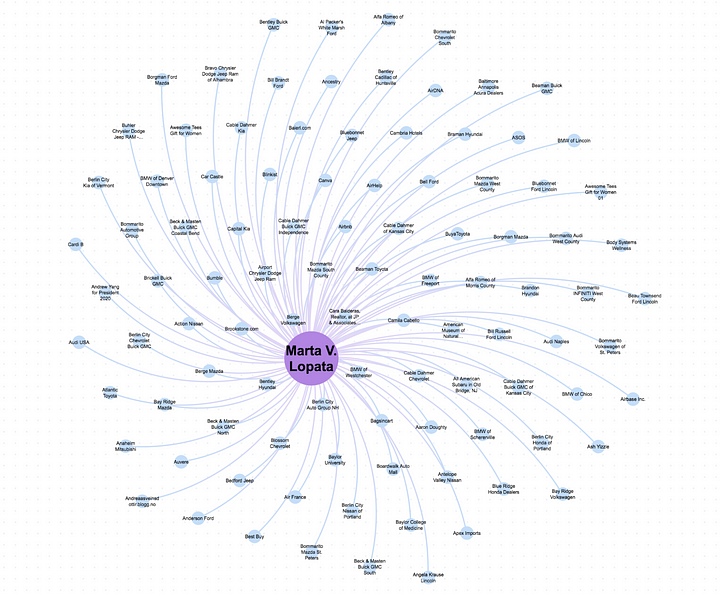
\includegraphics[width=0.7\textwidth]{img/facebook_graph.png}
          \caption{Reklama, kuri mato „Facebook“ vartotojas \cite{medium_article}}
          \label{fig:nodes}
    \end{figure}
\end{frame}

\begin{frame}[fragile]{Facebook santykių grafas}
    \begin{figure}[htbp]
          \centering
          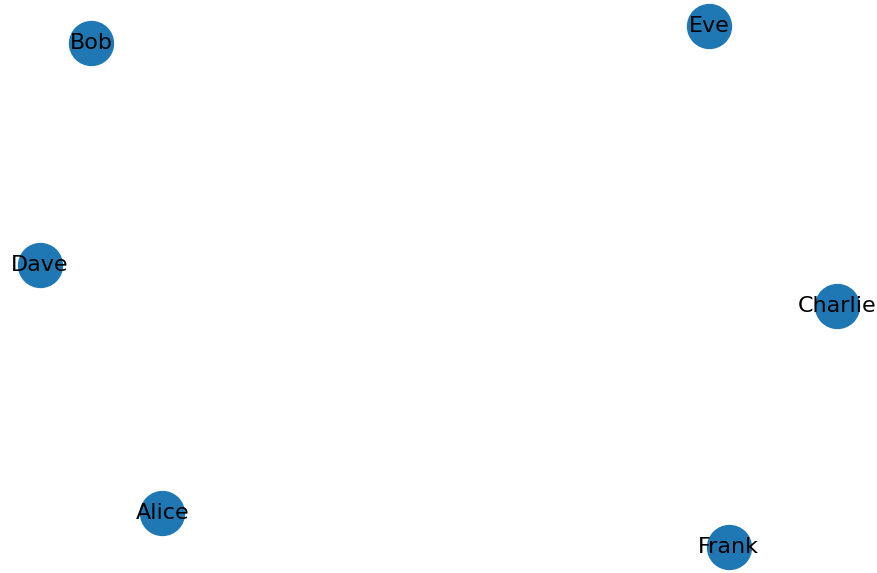
\includegraphics[width=1\textwidth]{img/nodes.png}
          \caption{Grafas, kur žmones reprezentuoja taškai}
          \label{fig:nodes}
    \end{figure}
\end{frame}

\begin{frame}[fragile]{Facebook santykių grafas} 
    \begin{figure}[htbp]
          \centering
          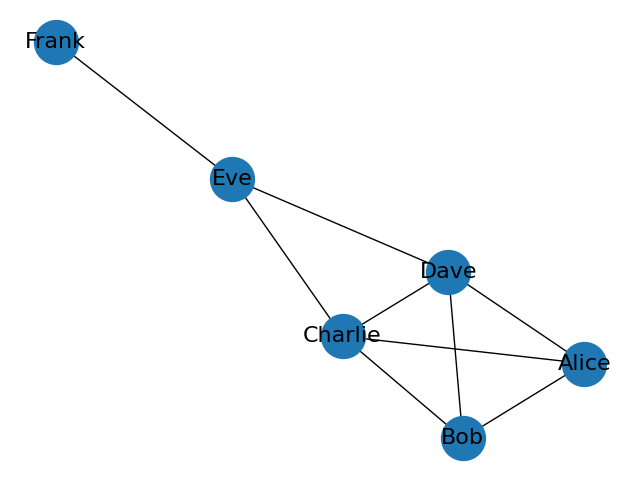
\includegraphics[width=0.8\textwidth]{img/vertex.png}
          \caption{Grafas, briaunos reprezentuoja draugystes tarp žmonių}
          \label{fig:vertex}
    \end{figure}
\end{frame}

\section{RDF modelis}

\begin{frame}[fragile]{Apibrėžimas}
    Resource Description Framework (RDF) yra W3C\footnote{W3C yra tarptautinė organizacija, kuri vysto ir skatina interneto standartus.} sukurtas semantinio interneto standartas, skirtas struktūrizuotų metaduomenų aprašymui. RDF turi savo kalbą, RDF Schema (RDFS), ir semantikos aprašymą OWL\footnote{OWL yra kalba, skirta apibrėžti sąvokas, taisykles ir santykius tarp objektų internete.} \cite{wiki:rdf}. RDF grafas yra sudarytas iš trijų teiginių sakinio, pavadinto "triple", kuriame yra subjektas, predikatas ir objektas ir kiekvieną "triple" galima identifikuoti unikaliu URI.
     \begin{figure}[htbp]
          \centering
          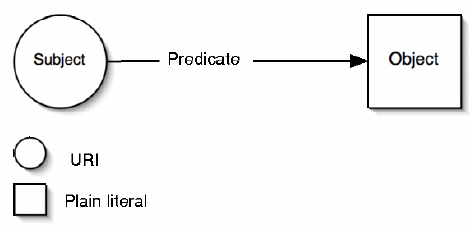
\includegraphics[width=0.6\textwidth]{img/rdf_triple.png}
          \caption{RDF triplas \cite{distributed_search}}
          \label{fig:vertex}
    \end{figure}
\end{frame}

\begin{frame}[fragile]{RDF triplo pavyzdis}
    Vilnius yra Lietuvos sostinė RDF triplas:
    \begin{enumerate}
        \item Subjektas: Vilnius
        \item Predikatas: yra sostinė
        \item Objektas: Lietuva
    \end{enumerate}

    Teiginio RDF modelis:
    \begin{lstlisting}[captionpos=b, caption=Teiginio RDF modelis, label=lst:rdf,
    basicstyle=\ttfamily\scriptsize,frame=single,breaklines=true]
    @prefix ex: <http://example.com/> .
    @prefix rdf: <http://www.w3.org/1999/02/22-rdf-syntax-ns#> .
    
    ex:Vilnius rdf:type rdf:Resource .
    ex:Lietuva rdf:type rdf:Resource .
    ex:Vilnius ex:yraSostine ex:Lietuva .
    \end{lstlisting}
\end{frame}


\section{SPARQL užklausų kalba}

\begin{frame}[fragile]{Apibrėžimas}
    SPARQL užklausų kalba, tai yra semantinė užklausų kalba duomenų bazių sistemoms, skirta gauti ir manipuliuoti duomenimis, saugomais RDF formatu \cite{wiki:sparql}.
\end{frame}

\subsection{SPARQL sintaksė}

\begin{frame}[fragile]{RDFo pavyzdis}
    Žmonės ir jų adresai
    \begin{lstlisting}[captionpos=b, caption=Žmonių RDF, label=lst:rdf1,
    basicstyle=\ttfamily\scriptsize,frame=single,breaklines=true]
    <http://example.org/person1> ex:hasName "John".
    <http://example.org/person1> ex:hasAge 25.
    <http://example.org/person2> ex:hasName "Mary".
    <http://example.org/person2> ex:hasAge 30.
    <http://example.org/person3> ex:hasName "Peter".
    <http://example.org/person3> ex:hasAge 35.
    \end{lstlisting}

    \begin{lstlisting}[captionpos=b, caption=Adresų RDF, label=lst:rdf2,
    basicstyle=\ttfamily\scriptsize,frame=single,breaklines=true]
    <http://example.org/person1> ex:hasAddress "123 Main St".
    <http://example.org/person2> ex:hasAddress "456 Park Ave".
    <http://example.org/person3> ex:hasAddress "789 Elm St".
    \end{lstlisting}
\end{frame}

\begin{frame}[fragile]{SPARQL užklausos pavyzdis}
    Informaciją apie žmones ir jų adresus, kurie yra vyresni nei 25 metai
    \begin{lstlisting}[captionpos=b, caption=Informaciją apie žmones ir jų adresus, label=lst:sparql, basicstyle=\ttfamily\scriptsize,frame=single]
    PREFIX ex: <http://example.org/>
    SELECT ?person ?name ?age ?address
    WHERE {
      ?person ex:hasName ?name .
      ?person ex:hasAge ?age .
      ?person ex:hasAddress ?address .
      FILTER (?age > 25)
    }
\end{lstlisting}


\begin{table}[h]
\centering
\begin{tabular}{|c|c|c|c|}
    \hline
    person & name & age & address \\
    \hline
    <http://example.org/person2> & Mary & 30 & 456 Park Ave \\
    <http://example.org/person3> & Peter & 35 & 789 Elm St \\
    \hline
    \end{tabular}
    \caption{Parinkti asmenys}
\end{table}

\end{frame}

\section{Žinių grafo pavyzdžio aprašymas}

\begin{frame}[fragile]{Žinių grafas}
    \begin{figure}[htbp]
          \centering
          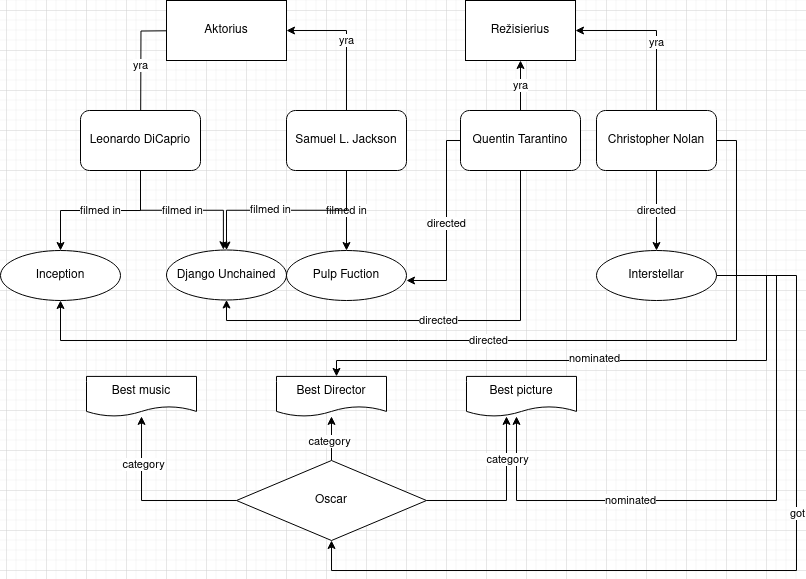
\includegraphics[width=0.9\textwidth]{img/grafas.png}
          \caption{Žinių grafas}
          \label{fig:vertex}
    \end{figure}
\end{frame}

\begin{frame}[fragile]{RDF modelio sąvokos}
    \begin{lstlisting}[captionpos=b, caption=RDF modelio sąvokos, label=lst:sparql,
   basicstyle=\ttfamily\scriptsize,frame=single]
    @prefix rdf: <http://www.w3.org/1999/02/22-rdf-syntax-ns#> .
    @prefix rdfs: <http://www.w3.org/2000/01/rdf-schema#> .
    @prefix ex: <http://example.com/> .
    
    ex:Aktorius rdf:type rdfs:Class .
    ex:Reziserius rdf:type rdfs:Class .
    ex:LeonardoDicaprio rdf:type ex:Aktorius .
    ex:SamuelLJackson rdf:type ex:Aktorius .
    ex:QuentinTarantino rdf:type ex:Reziserius .
    ex:ChristopherNolan rdf:type ex:Reziserius .
    ex:Inception rdf:type rdfs:Class .
    ex:DjangoUnchained rdf:type rdfs:Class .
    ex:PulpFiction rdf:type rdfs:Class .
    ex:Interstellar rdf:type rdfs:Class .
    ex:BestMusic rdf:type rdfs:Class .
    ex:BestDirector rdf:type rdfs:Class .
    ex:BestPicture rdf:type rdfs:Class .
    ex:Oscar rdf:type rdfs:Class .
    \end{lstlisting}
\end{frame}

\begin{frame}[fragile]{RDF modelio ryšiai}
    \begin{lstlisting}[captionpos=b, caption=RDF modelio ryšiai, label=lst:sparql,
   basicstyle=\ttfamily\scriptsize,frame=single]
    ex:LeonardoDicaprio ex:filmedIn ex:Inception .
    ex:LeonardoDicaprio ex:filmedIn ex:DjangoUnchained .
    ex:SamuelLJackson ex:filmedIn ex:DjangoUnchained .
    ex:SamuelLJackson ex:filmedIn ex:PulpFiction .
    ex:QuentinTarantino ex:directed ex:PulpFiction .
    ex:ChristopherNolan ex:directed ex:Inception .
    ex:ChristopherNolan ex:directed ex:Interstellar .
    ex:Interstellar ex:nominated ex:BestMusic .
    ex:Interstellar ex:nominated ex:BestDirector .
    ex:Interstellar ex:got ex:Oscar .
    ex:Oscar ex:hasCategory ex:BestMusic .
    ex:Oscar ex:hasCategory ex:BestDirector .
    ex:Oscar ex:hasCategory ex:BestPicture .
    \end{lstlisting}
\end{frame}

\begin{frame}[fragile]{RDF modelio grafas}
    \begin{figure}[htbp]
        \centering
        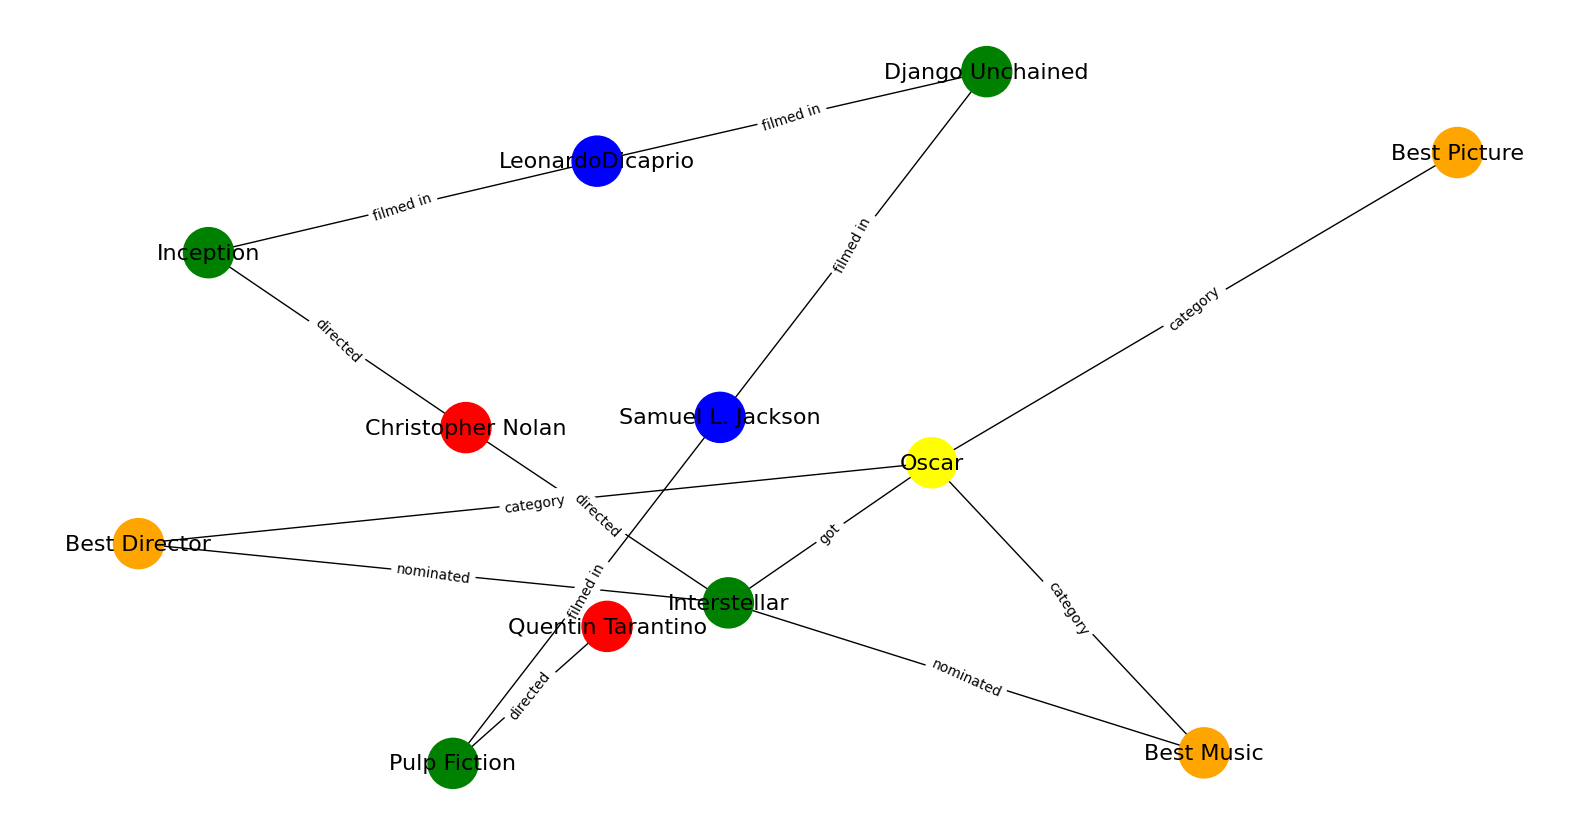
\includegraphics[width=1\textwidth]{img/last_graph_rdf.png}
        \caption{Žinių grafas, naudojant networkX ir Matplotlib biblioteka}
        \label{fig:last_graph_rdf}
    \end{figure}
\end{frame}

\begin{frame}[fragile]{Klausimai}
    \begin{enumerate}
        \item Ar gavo Christopherio Nolano filmas "Interstellar" gavo Oscar už nominacija best picture?
        \item Kokiame filme vaidino Samuel L. Jackson?
        \item Ar Christopherio Nolano filmas "Interstellar" gavo Oscar?
    \end{enumerate}
\end{frame}

\begin{frame}[fragile]{Užklausa 1}
    \begin{lstlisting}[captionpos=b, caption=Ar Christopherio Nolano filmas "Interstellar" gavo Oscar už nominacija best picture?, label=lst:sparql,
       basicstyle=\ttfamily\scriptsize,frame=single]
    PREFIX rdf: <http://www.w3.org/1999/02/22-rdf-syntax-ns#>
    PREFIX rdfs: <http://www.w3.org/2000/01/rdf-schema#>
    PREFIX ex: <http://example.com/>
    
    SELECT ?result WHERE {
      ex:Interstellar ex:got ex:Oscar .
      ex:Oscar ex:hasCategory ex:BestPicture .
      ex:Oscar ex:hasCategory ?result .
    }
    \end{lstlisting}
\end{frame}

\begin{frame}[fragile]{Užklausa 2}
    \begin{lstlisting}[captionpos=b, caption=Kokiame filme vaidino Samuel L. Jackson?, label=lst:sparql,
       basicstyle=\ttfamily\scriptsize,frame=single]
    PREFIX rdf: <http://www.w3.org/1999/02/22-rdf-syntax-ns#>
    PREFIX ex: <http://example.com/>
    
    SELECT ?filmas
    WHERE {
      ex:SamuelLJackson ex:filmedIn ?filmas .
    }
    \end{lstlisting}
\end{frame}

\begin{frame}[fragile]{Užklausa 3}
    \begin{lstlisting}[captionpos=b, caption=Ar Christopherio Nolano filmas "Interstellar" gavo Oscar?, label=lst:sparql,
       basicstyle=\ttfamily\scriptsize,frame=single]
    PREFIX rdf: <http://www.w3.org/1999/02/22-rdf-syntax-ns#>
    PREFIX ex: <http://example.com/>
    
    SELECT ?oscar
    WHERE {
      ex:Interstellar ex:got ?oscar .
      ?oscar ex:hasCategory ex:BestPicture .
    }
    \end{lstlisting}
\end{frame}

\section{Rezultatai ir išvados}

\begin{frame}[allowframebreaks]{Šaltiniai}
  \printbibliography[heading=none]
\end{frame}

\end{document}
